
%(BEGIN_QUESTION)
% Copyright 2010, Tony R. Kuphaldt, released under the Creative Commons Attribution License (v 1.0)
% This means you may do almost anything with this work of mine, so long as you give me proper credit

A process patented by Siemens for forming rods of ultra-pure silicon used as feedstock for manufacturing solar (photovoltaic) cells is called the ``TCS method.''  ``TCS'' stands for Tri-Chloro-Silane, and it is a gas with the chemical formula HSiCl$_{3}$.

The process uses a thread of silicon suspended between two electrical contacts.  Electric current passed through the silicon thread heats it up to a high temperature, and then the TCS gas (plus hydrogen gas) is admitted into the vessel called a ``CVD reactor'' (Chemical Vapor Deposition) at a pressure of 6 bar (gauge).  There, the gases contact the silicon thread and react for form pure silicon (Si) and hydrochloric acid (HCl), leaving the silicon as new layers accumulated on the thread.  Eventually the thread grows thicker until it becomes a solid rod of silicon ready to process into solar cells.  The acid vapors exit the reactor, along with unreacted TCS and hydrogen gases:

$$\includegraphics[width=15.5cm]{i00574x01.eps}$$

Balance this chemical equation showing the desired reaction forming new layers of silicon on the thread inside the CVD reactor:

$$\hbox{HSiCl}_3 + \hbox{H}_2 \rightarrow \hbox{Si} + \hbox{HCl}$$

Also, express the reactor gas pressure in units of PSIG.

\vskip 20pt \vbox{\hrule \hbox{\strut \vrule{} {\bf Suggestions for Socratic discussion} \vrule} \hrule}

\begin{itemize}
\item{} Based on the description of the process, do you suspect the reaction is exothermic or endothermic, or is there too little information given to tell?
\item{} How safe would you consider some of these compounds used in silicon manufacturing, with respect to human exposure?
\end{itemize}

\underbar{file i00574}
%(END_QUESTION)





%(BEGIN_ANSWER)


%(END_ANSWER)





%(BEGIN_NOTES)

This reaction is so easy to balance that we do not need to use algebra.  All we need to do is have {\it three} acid molecules on the right-hand side to balance out the three hydrogen atoms and three chlorine atoms on the left.

$$\hbox{HSiCl}_3 + \hbox{H}_2 \rightarrow \hbox{Si} + 3\hbox{HCl}$$

\vskip 10pt

6 bar (gauge) = 87 PSIG

\vskip 10pt

Information for this question came from Emerson's ``Process Solutions Guide'' on the Siemens TCS Method, document number MC-001192.

%INDEX% Chemistry, stoichiometry: reaction quantities
%INDEX% Process: silane combustion

%(END_NOTES)


